\documentclass{article}
% \usepackage{xeCJK}
\usepackage{amsmath}
\usepackage{amssymb}
\usepackage{mathrsfs}
\usepackage{xcolor}
\usepackage{bm}
\usepackage{hyperref}
\usepackage{graphicx}
\usepackage{subcaption}
\usepackage{float}
\usepackage{multicol}
\usepackage[ruled,linesnumbered]{algorithm2e}

\bibliographystyle{plain}
\setlength{\parindent}{2em}
\usepackage{geometry}
\geometry{a4paper, left=2.54cm, right=2.54cm, top=3.18cm, bottom=3.18cm}

% 设置文章行距
% \renewcommand{\baselinestretch}{1.5}

% define reference format
\hypersetup{
    colorlinks=true,
    linkcolor=blue,
    urlcolor=blue,
    citecolor=blue,
    linkbordercolor=white
}

\title{\textbf{Chemotactic Chiral Active Matter}}
\author{Yichen Lu}

\begin{document}

\maketitle

\tableofcontents

\newpage
\section{Models}
\subsection{Definitions}
\subsubsection{Self-propelled dynamics}

\begin{subequations}
    \begin{align}
    \dot{x}_i&=v\cos \theta _i\;,
    \\
    \dot{y}_i&=v\sin \theta _i\;,
    \end{align}
    \label{eq:dotxy}
\end{subequations}

\subsubsection{Polar alignment dynamics}
\begin{itemize}
    \item Additive coupling: 
    \begin{equation}
        \label{eq:additionalCouplingDotTheta}
        \dot{\theta}_i=\omega _i+K\sum_{j=1}^{N}f\left( r_{ij} \right)\sin \left( \theta _j-\theta _i+\alpha \right)\;,
    \end{equation}
    \item Mean-field coupling by oscillator number:
    \begin{equation}
        \label{eq:swarmalatorDotTheta}
        \dot{\theta}_i=\omega _i+\frac{K}{N}\sum_{j=1}^N{f}\left( r_{ij} \right) \sin \left( \theta _j-\theta _i+\alpha \right) \;,
    \end{equation}
    which is similar to the swarmalator model.
    % \item Mean-field coupling by oscillator density:
    % \begin{equation}
    %     \dot{\theta}_i=\omega _i+\frac{KL^2}{\pi d_{0}^{2}N}\sum_{j=1}^N{f}\left( r_{ij} \right) \sin \left( \theta _j-\theta _i+\alpha \right) \;,
    % \end{equation}
    % where $d_0$ is the radius of the interaction circle.
\end{itemize}
Here,  $f\left( r_{ij} \right)$ is a function of $r=\left| \mathbf{r}_i-\mathbf{r}_j \right|$, and $K$ is the coupling strength. 
The function $f\left( r \right)$ can be defined as
\begin{enumerate}
    \item $f_H\left( r \right)=H\left( d_0-r \right),\;r_0>0$;
    \item $f_E\left( r \right)=e^{-\frac{r}{d_0}},\;r_0>0$.
\end{enumerate}
The natural frequencies $\omega_i$ are distributed with following two cases:
\begin{enumerate}
    \item \textbf{Single-chiral swarmalators:} The natural frequencies $\omega_i$ are distributed in $U\left( \omega _{\min},\omega _{\max} \right)$ for all swarmalators and $\omega _{\min}\omega _{\max}>0$.
    
    \item \textbf{Double-chiral swarmalators:} The frequencies are distributed in two symmetric uniform distributions, representing two types of chirality. Exactly half of the swarmalators have natural frequencies $\omega_i \sim U\left( \omega _{\min},\omega _{\max} \right)$ and the other half have natural frequencies $\omega_i \sim U\left( -\omega _{\max},-\omega _{\min} \right)$.
\end{enumerate}

\subsubsection{Chemotactic dynamics}

Consider two chemical fields $u\left( \mathbf{r},t \right), v\left( \mathbf{r},t \right)$ that are produced by the ensemble of two symmetrically chiral swarmalators. Swarmalators interact with the chemical field and move towards/against the regions with higher concentration, which can be described by the following equation ($i=1, 2, \dots, N$):
\begin{subequations}
    \begin{align}
        \dot{\mathbf{r}}_{i}^{s}&=v\mathbf{p}\left(\theta_{i}^{s}\right)\\
        \dot{\theta}_{i}^{s}&=\omega _{i}^{s}+\alpha ^{s}\mathbf{p}_{i}^{s}\times \nabla u+\beta ^{s}\mathbf{p}_{i}^{s}\times \nabla v
    \end{align}
\end{subequations}
where $\alpha, \beta _{i}^{s}$ denote the ‘chemotactic’ coupling strength and $\mathbf{p}\left(\theta\right)=(\cos \theta,\sin \theta )$ is the unit vector pointing in the direction of the $i$-th swarmalator, $s\in\{p, n\}$ denotes the two chiral species. Here, we used the notation $\mathbf{a}\times\mathbf{b}=a_1 b_2-a_2 b_1$.

These two fields evolve as
\begin{subequations}
    \begin{align}
    \dot{u}&=k_0\sum_{j=1}^N{\delta \left( \mathbf{r}-\mathbf{r}_{j}^{p} \right)}-k_du+D_u\nabla ^2u\;,\\
    \dot{v}&=k_0\sum_{j=1}^N{\delta \left( \mathbf{r}-\mathbf{r}_{j}^{n} \right)}-k_dv+D_v\nabla ^2v\;,
    \end{align}
\end{subequations}
where $S_+$ and $S_-$ are the sets of two chiral swarmalators, $k_0$ is the production rate, $k_d$ is the decay rate, $D_{u,v}$ are the diffusion coefficients.

\subsubsection{Mixed phase dynamics}
\begin{subequations}
    \begin{align}
        \dot{\mathbf{r}}_i&=v\mathbf{p}_i\\
        \dot{\theta}_i&=\omega _i+\beta _{i}^{u}\mathbf{p}_i\times \nabla u+\beta _{i}^{v}\mathbf{p}_i\times \nabla v+\frac{K}{N}\sum_{j=1}^N{f}\left( \left| \mathbf{r}_j-\mathbf{r}_i \right| \right) \sin \left( \theta _j-\theta _i \right) \;,
    \end{align}
\end{subequations}

\subsubsection{General Chemotactic Model For Two Species}
\textcolor{red}{Type 1:}
\begin{subequations}
    \begin{align}
        &\dot{\mathbf{r}}_{i}^{1,2}=v\mathbf{p}\left( \theta _{i}^{1,2} \right) -\sum_{j\in A_{i}^{1,2}}{\mathbf{I}_{ij}^{1,2}\;,}\\
        &\dot{\theta}_{i}^{1,2}=\left| \nabla c_{1,2} \right|\sin \left( \varphi _{c_{1,2}}-\theta _{i}^{1,2} \right) +F\left( \theta ,\mathbf{r} \right) \;,\\
        &\dot{c}_1=D_1\nabla ^2c_1+F_1\left( c_1,c_2 \right) \sum_{j=1}^N{\delta \left( \mathbf{r}-\mathbf{r}_{j}^{1} \right) \;,}\\
        &\dot{c}_2=D_2\nabla ^2c_2+F_2\left( c_1,c_2 \right) \sum_{j=1}^N{\delta \left( \mathbf{r}-\mathbf{r}_{j}^{2} \right) \;,}
    \end{align}
\end{subequations}
where $\mathbf{I}_{ij}^{1,2}=\frac{\mathbf{r}_j-\mathbf{r}_{i}^{1,2}}{|\mathbf{r}_j-\mathbf{r}_{i}^{1,2}|^{2}}$, $\varphi _{c_{1,2}}=\arctan \left( \frac{\partial _yc_{1,2}}{\partial _xc_{1,2}} \right) $ and $A_{i}^{1,2}=\left\{ j\mid r_c\geqslant | \mathbf{r}_j-\mathbf{r}_{i}^{1,2} | \right\}$.

\noindent Type 2:
\begin{subequations}
    \begin{align}
        &\dot{\mathbf{r}}_{i}^{1,2}=v\mathbf{p}\left( \theta _{i}^{1,2} \right) +\alpha _{1,2}\nabla c_{1,2}-\sum_{j\in A_{i}^{1,2}}{\mathbf{I}_{ij}^{1,2}\;,}\\
        &\dot{\theta}_{i}^{1,2}=F\left( \theta ,\mathbf{r} \right) \;,\\
        &\dot{c}_1=D_1\nabla ^2c_1+F_1\left( c_1,c_2 \right) \sum_{j=1}^N{\delta \left( \mathbf{r}-\mathbf{r}_{j}^{1} \right) \;,}\\
        &\dot{c}_2=D_2\nabla ^2c_2+F_2\left( c_1,c_2 \right) \sum_{j=1}^N{\delta \left( \mathbf{r}-\mathbf{r}_{j}^{2} \right) \;,}
    \end{align}
\end{subequations}

\subsubsection{Chemotactic Model with Lotka-Volterra Functions}
Let $F_1\left( c_1,c_2 \right)=c_1\left( k_1-k_2c_2 \right)$ and $F_2\left( c_1,c_2 \right)=c_2\left( k_3c_1-k_4 \right)$, where $k_1,k_2,k_3,k_4$ are constants.

\begin{subequations}
    \begin{align}
        &\dot{\mathbf{r}}_{i}^{1,2}=v\mathbf{p}\left( \theta _{i}^{1,2} \right) -\sum_{j\in A_{i}^{1,2}}{\mathbf{I}_{ij}^{1,2}\;,}\\
        &\dot{\theta}_{i}^{1,2}=\left| \nabla c_{1,2} \right|\sin \left( \varphi _{c_{1,2}}-\theta _{i}^{1,2} \right) +F\left( \theta ,\mathbf{r} \right) \;,\\
        &\dot{c}_1=D_1\nabla ^2c_1+c_1\left( k_1-k_2c_2 \right) \sum_{j=1}^N{\delta \left( \mathbf{r}-\mathbf{r}_{j}^{1} \right) \;,}\\
        &\dot{c}_2=D_2\nabla ^2c_2+c_2\left( k_3c_1-k_4 \right) \sum_{j=1}^N{\delta \left( \mathbf{r}-\mathbf{r}_{j}^{2} \right) \;,}
    \end{align}
\end{subequations}

\section{Behaviors}
\begin{figure}
    \centering
    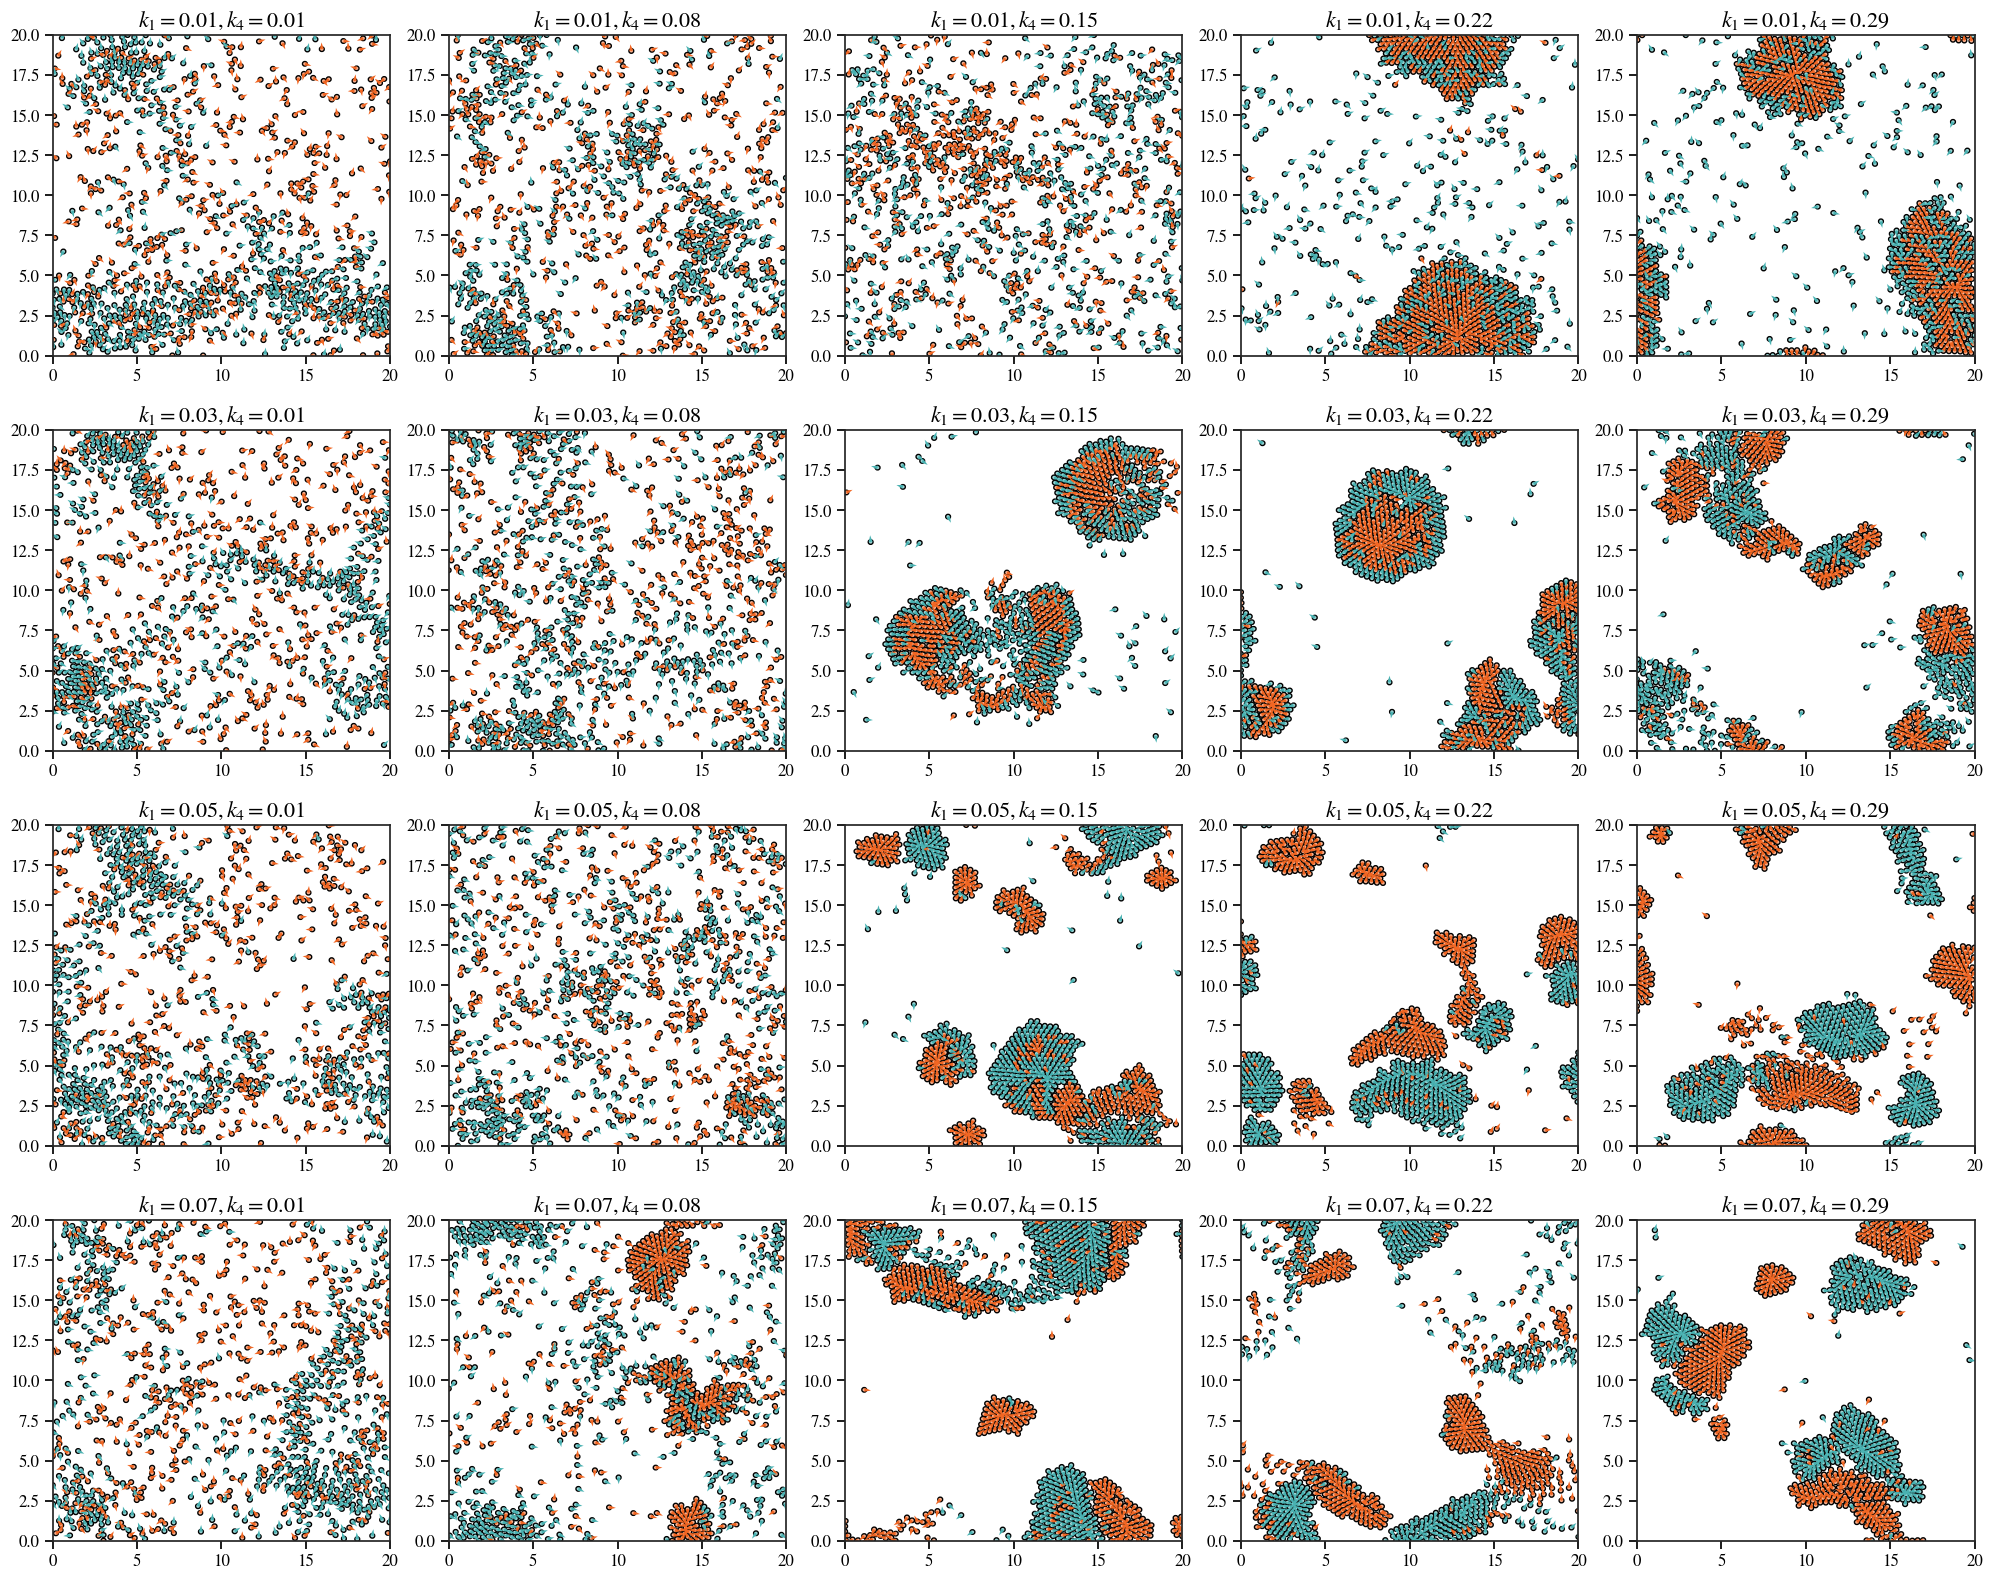
\includegraphics[width=\textwidth]{figs/bigGraphParticle_k23_0.5.png}
\end{figure}


\section{Continuum model}
The continuum model can be derived from a Boltzmann-like approach for the probability density $P(\mathbf{r}, \theta, t)$ of finding a particle at position $\mathbf{r}$ with orientation $\theta$ at time $t$. 




% \bibliography{ref}

\end{document}